\documentclass[10pt,twocolumn]{article}

\usepackage[T1]{fontenc}
\usepackage[utf8]{inputenc}
\usepackage{lmodern}
\usepackage[margin=0.66in,columnsep=0.24in]{geometry}
\usepackage{amsmath,amssymb}
\usepackage{booktabs}
\usepackage{graphicx}
\usepackage{microtype}
\usepackage[numbers,sort&compress]{natbib}
\usepackage{enumitem}
\usepackage{xcolor}
\usepackage{url}
\usepackage[hidelinks]{hyperref}
\usepackage{balance}

\graphicspath{{figures/}}
\setlist{nosep,leftmargin=*}
\setlength{\parindent}{1em}
\setlength{\parskip}{0pt}
\setlength{\textfloatsep}{7pt plus 2pt minus 2pt}
\setlength{\floatsep}{6pt plus 2pt minus 2pt}
\setlength{\intextsep}{6pt plus 2pt minus 2pt}
\setlength{\tabcolsep}{3.5pt}
\renewcommand{\arraystretch}{1.06}
\renewcommand{\topfraction}{0.95}
\renewcommand{\bottomfraction}{0.90}
\renewcommand{\textfraction}{0.05}
\renewcommand{\floatpagefraction}{0.85}

\newcommand{\dlt}{\Delta}
\newcommand{\ph}{\phi}
\newcommand{\wmax}{w_{\max}}
\newcommand{\pp}{\text{pp}}
\newcommand{\ntrain}{n_{\mathrm{train}}}
\newcommand{\ours}{\textsc{DijkWalk}}
\newcommand{\code}[1]{\texttt{\small #1}}
\newcommand{\hashcode}[2]{\texttt{\scriptsize #1\hspace{0pt}#2}}

\title{\vspace{-1.4em}\bfseries
When Does Directional Reward Shaping Matter?\\[-0.2em]
\large Same Dijkstra Regret, Two Learning Paradigms, One Graph-Walking Task}
\author{Anonymous Author(s)}
\date{}

\begin{document}
\maketitle
\vspace{-1.8em}

\begin{abstract}
Potential-based shaping can preserve optimal policies, but that invariance
result does not predict finite-budget learning speed or tell us whether an
exact directional signal should enter as a reward or a supervised loss.  We
study shortest-path execution on connected weighted graphs under a strictly
local observation.  At each node, a policy sees at most the eight cheapest
incident edges and must reach a hidden target.  Dijkstra's potential gives the
exact one-step regret
$\dlt(u,v)=w(u,v)+\ph(v)-\ph(u)$.
We expose the same quantity either as the reinforcement-learning reward
$-\dlt/\wmax$ or as the weight in a teacher-forced soft-KL objective.  Models
are matched at two parameter scales and two estimated-compute budgets, trained
with three seeds, and evaluated by both greedy and sampled decoding on three
hash-pinned 1,000-graph suites.

At the 25M match, sampled RL attains 90.8\% and 87.6\% far-out-of-distribution
(OOD) success at the small and large scales, versus 12.8\% and 31.3\% for
supervision.  RL also makes fewer backward moves and yields substantially
cheaper successful walks.  The predeclared cross-paradigm gate passes in 24
success cells, 24 optimality-gap cells, and six size-degradation comparisons.
A separate 162-run shaping phase diagram produces a coherent 8--12 point
advantage on large cold-start graphs with tight horizons, but no cell reaches
its predeclared 15-point gate: an honest null.  Finally, sampled MLP and LSTM
policies retain 90.9\% and 93.6\% success at 24 times the largest training
size, while a Transformer falls to 56.1\%.  High random-walk success and
near-universal two-cycles show why reachability, efficiency, and decoding must
be reported jointly.  The results support a narrow conclusion: for this local
graph walker, the learning interface and induced state distribution matter
more than merely possessing an exact directional signal.
\end{abstract}

\section{Introduction}

Dijkstra's algorithm provides unusually clean supervision for testing learned
graph search.  If
$\ph(x)=d(x,\mathrm{target})$ is the exact shortest-path potential, every
candidate move $u\!\rightarrow\!v$ has nonnegative regret
\begin{equation}
  \dlt(u,v)=w(u,v)+\ph(v)-\ph(u)\geq 0,
  \label{eq:regret}
\end{equation}
with equality precisely for a shortest-path-consistent move.  The same scalar
can grade an expert action, shape an RL reward, or remain only an evaluation
diagnostic.  This lets us ask a controlled question obscured in most learned
search comparisons: what changes when the information is held fixed but its
learning interface changes?

Potential-based reward shaping (PBRS) can preserve an MDP's optimal policies
under its standard discounted construction \citep{ng1999}.  This theorem is
silent about finite-budget optimization and does not equate teacher-forced
learning with on-policy interaction.  A supervised executor trains on expert
states.  An RL walker trains on states induced by its own errors, detours, and
recoveries.  Holding the local signal fixed isolates this difference more
cleanly than comparing unrelated rewards and targets.

We make four contributions.  First, we compare PPO-based RL and soft-KL
supervision on identical frozen graph suites at two closely matched parameter
scales and two approximate multiply--accumulate (MAC) budgets.  Second, we
predeclare and execute a reward-shaping phase diagram over graph size, horizon,
and terminal bonus; its null is retained rather than tuned away.  Third, we
evaluate size generalization through $n=768$, 24 times the largest training
graph, with classical controls and cycle diagnostics.  Fourth, we provide a
deterministic seed path, hash-pinned suites, complete three-seed aggregates,
and a behavior-preserving vectorized environment.

Our claims are deliberately narrower than ``RL beats supervision'' or
``the network learns Dijkstra.''  They concern local-observation graph walkers,
the exact regret in Equation~\eqref{eq:regret}, and a fixed family of connected random
weighted graphs.  Even in that controlled setting, success alone is
misleading: a uniform random valid walk exceeds 80\% success under a generous
$4n$ horizon while taking paths hundreds of times more costly than optimal.

\section{Related Work}

\paragraph{Reward shaping.}
PBRS characterizes policy-invariant reward transformations
\citep{ng1999}.  Later work learns when or how strongly to use shaping signals
\citep{hu2020,gupta2023}, while hindsight methods alter the effective learning
signal after failed trajectories \citep{andrychowicz2017}.  We do not learn a
potential: Dijkstra supplies the exact one.  Our empirical question is when
that exact potential difference improves a fixed finite-budget learner.

\paragraph{Neural algorithmic reasoning.}
The CLRS benchmark and related neural executors emphasize out-of-distribution
size generalization, intermediate supervision, and algorithmic traces
\citep{velickovic2020,velickovic2022,ibarz2022,bevilacqua2023,dudzik2022}.
GNARL independently reframes neural algorithmic reasoning through RL
\citep{schutz2025}.  Our distinction is the controlled use of the same
per-decision Dijkstra regret as either a supervised weight or an RL reward on
the same evaluation instances.

\paragraph{Learned search and solvers.}
Differentiable planning \citep{yonetani2021}, learned SAT procedures
\citep{yolcu2019,selsam2019}, and learned combinatorial heuristics
\citep{khalil2017} motivate separating completion from search efficiency.
Instruction-pointer executors similarly expose the importance of execution
state \citep{bieber2020}.  We therefore report success, successful-path cost,
backward motion, two-cycles, and both stochastic and deterministic decoding.

\section{Task and Protocol}
\label{sec:protocol}

\subsection{Local graph walking}

Each episode samples a connected weighted graph $G=(V,E)$, source $s$, and
target $t$.  At the current node $u$, the policy observes $K=8$ neighbor slots.
Each slot contains a validity bit, normalized edge weight, visited bit, and
target bit.  Two global scalars encode normalized rollout progress and clipped
graph size.  The policy receives neither the global adjacency matrix nor
$\ph$.  Nodes of degree greater than $K$ expose the $K$ cheapest edges with a
deterministic weight--node identifier tie break.

Training begins on $n\in[8,16]$ and normally expands to $n=32$ after rolling
success exceeds 0.9.  The default episode horizon is $4n$.  Action masks are
computed from observed valid flags; invalid-action rate is a hard integrity
metric and equals zero in every reported condition.

\subsection{One regret, two interfaces}

The graded environment reward is
\begin{equation}
 r(u,v)=
 \frac{-w(u,v)+\beta\!\left[\ph(u)-\ph(v)\right]}{\wmax}-c,
 \label{eq:reward}
\end{equation}
plus a terminal goal bonus.  At $\beta=1$ and ignoring the shared step cost,
Equation~\eqref{eq:reward} is exactly $-\dlt(u,v)/\wmax$.  The $\beta=0$ control still
pays edge and step costs; ``sparse'' is retained only as harness terminology.
A third reward gives a binary penalty whenever $\ph(v)>\ph(u)$.

The supervised sibling uses teacher forcing with a soft-KL objective whose
per-decision weights derive from the same Dijkstra regret.  Small and large
supervised models are matched to an RL LSTM and Transformer, respectively.
The comparison therefore fixes graph generation, local features, regret
definition, parameter scale, and approximate model MACs while allowing the
training state distribution and optimizer to differ.

\subsection{Policies and optimization}

RL policies use an MLP, recurrent LSTM, or slot-token Transformer encoder.
Q1 compares the LSTM and Transformer with their parameter-matched supervised
counterparts.  RL uses PPO with Muon at learning rate 0.015 and
$\gamma=0.995$.  The potential term in Equation~\eqref{eq:reward} is undiscounted, so we
claim the exact $\dlt$ identity but not exact discounted PBRS invariance for
the PPO objective.

All learned conditions use training seeds 42, 43, and 44.  The seed is applied
before model construction to Python, NumPy, PyTorch, PufferLib, action
sampling, and graph generation.  It appears in every checkpoint, curve,
manifest, and evaluation filename.

\subsection{Frozen evaluation and metrics}

Q1 uses three serialized suites of 1,000 graphs each: train scale
$n\in[16,32]$, near OOD $n\in[33,48]$, and far OOD $n\in[64,96]$.
Both argmax (greedy) and categorical (sampled) decoding are evaluated.
Success is target attainment.  Optimality gap is
\begin{equation}
  \mathrm{gap}(\tau)=
  \frac{\sum_{(u,v)\in\tau} w(u,v)}{d(s,t)}
\end{equation}
and is defined only on successful episodes.  Backward rate is the fraction of
valid moves with $\ph(v)>\ph(u)$.  We also record whether a trajectory
contains a two-cycle $u\!\rightarrow\!v\!\rightarrow\!u$.

\subsection{Predeclared decision gates}

Q1 is interesting if either paradigm differs by more than five success points
or 0.5 optimality gap in any matched cell, or if train-to-OOD degradation
differs.  Q2 requires a $\geq15$ point graded-minus-$\beta{=}0$ success gap and
non-overlapping seed ranges.  Q3 requires one architecture to retain
$>80\%$ success at least $8\times$ beyond training size while another collapses,
or a ranking reversal.  These are practical effect-size gates, not post-hoc
$p$-value thresholds.

\section{Q1: Reward Versus Loss Weight}
\label{sec:q1}

\subsection{Matching}

\begin{table}[t]
\centering
\caption{Q1 parameter and estimated-compute matching.  Ratios are supervised
to RL MAC estimates and exclude environment and optimizer work.}
\label{tab:match}
\small
\begin{tabular}{@{}lrrrr@{}}
\toprule
Scale & RL params & Sup.\ params & 5M ratio & 25M ratio\\
\midrule
Small & 183,081 & 185,192 & 1.010 & 1.009\\
Large & 531,202 & 532,152 & 0.987 & 0.986\\
\bottomrule
\end{tabular}
\end{table}

Table~\ref{tab:match} shows close parameter and model-MAC matching.  The supervised
steps selected for the 5M and 25M matches are 200 and 1,000 at small scale,
and 1,500 and 7,500 at large scale.  We report those approximate matches
transparently rather than equating MACs with wall-clock or data exposure.

\subsection{Matched-compute results}

\begin{table*}[t]
\centering
\caption{Q1 at the 25M compute match.  Entries are three-seed means in the
form success (\%) / optimality gap / backward rate (\%).  Optimality gap is
conditional on success; lower gap and backward rate are better.}
\label{tab:q1main}
\footnotesize
\resizebox{\textwidth}{!}{%
\begin{tabular}{@{}lllccc@{}}
\toprule
Scale & Learner & Decode &
Train scale $n{=}16$--32 & Near OOD $n{=}33$--48 & Far OOD $n{=}64$--96\\
\midrule
Small & RL & greedy
 & 94.13 / 2.18 / 20.02 & 90.53 / 3.13 / 25.83 & 79.13 / 5.29 / 33.94\\
Small & RL & sampled
 & 97.23 / 2.43 / 19.88 & 95.77 / 3.70 / 25.69 & \textbf{90.80 / 6.77 / 33.41}\\
Small & supervised & greedy
 & 18.47 / 4.70 / 42.36 & 12.23 / 5.67 / 45.16 & 4.67 / 14.14 / 46.96\\
Small & supervised & sampled
 & 75.97 / 14.43 / 38.42 & 53.33 / 19.16 / 42.65 & 12.77 / 23.07 / 46.19\\
\midrule
Large & RL & greedy
 & 87.10 / 1.92 / 20.66 & 78.93 / 2.52 / 26.71 & 69.23 / 3.69 / 33.74\\
Large & RL & sampled
 & 96.37 / 2.52 / 20.21 & 92.53 / 3.46 / 26.18 & \textbf{87.57 / 6.04 / 33.63}\\
Large & supervised & greedy
 & 66.93 / 2.54 / 22.95 & 22.90 / 10.17 / 42.48 & 6.27 / 48.15 / 47.19\\
Large & supervised & sampled
 & 90.90 / 5.77 / 26.30 & 62.67 / 20.65 / 41.00 & 31.33 / 58.85 / 46.23\\
\bottomrule
\end{tabular}}
\end{table*}

Table~\ref{tab:q1main} contains the headline 25M comparison.  Sampled far-OOD
success is 90.80\% RL versus 12.77\% supervised at small scale, a
78.03-point difference.  At large scale it is 87.57\% versus 31.33\%, a
56.23-point difference.  Greedy decoding does not reverse the ordering:
far-OOD RL reaches 79.13\% and 69.23\%, while supervision reaches 4.67\% and
6.27\%.

The divergence grows with graph size.  Under sampled decoding, small-model
train-to-far success drops 6.43 points for RL but 63.20 for supervision.
Large-model drops are 8.80 and 59.57 points.  The three-seed ranges do not
overlap in either comparison.

Path behavior points in the same direction.  In the 25M far-OOD sampled cells,
RL backward rates are 33.41\% and 33.63\%, versus 46.19\% and 46.23\%.
Successful RL trajectories cost 6.77 and 6.04 times optimal, versus 23.07 and
58.85 for supervision.  Conditional gaps require care: a deceptively small
greedy gap may summarize only a few successful supervised episodes.

\begin{figure*}[t]
\centering
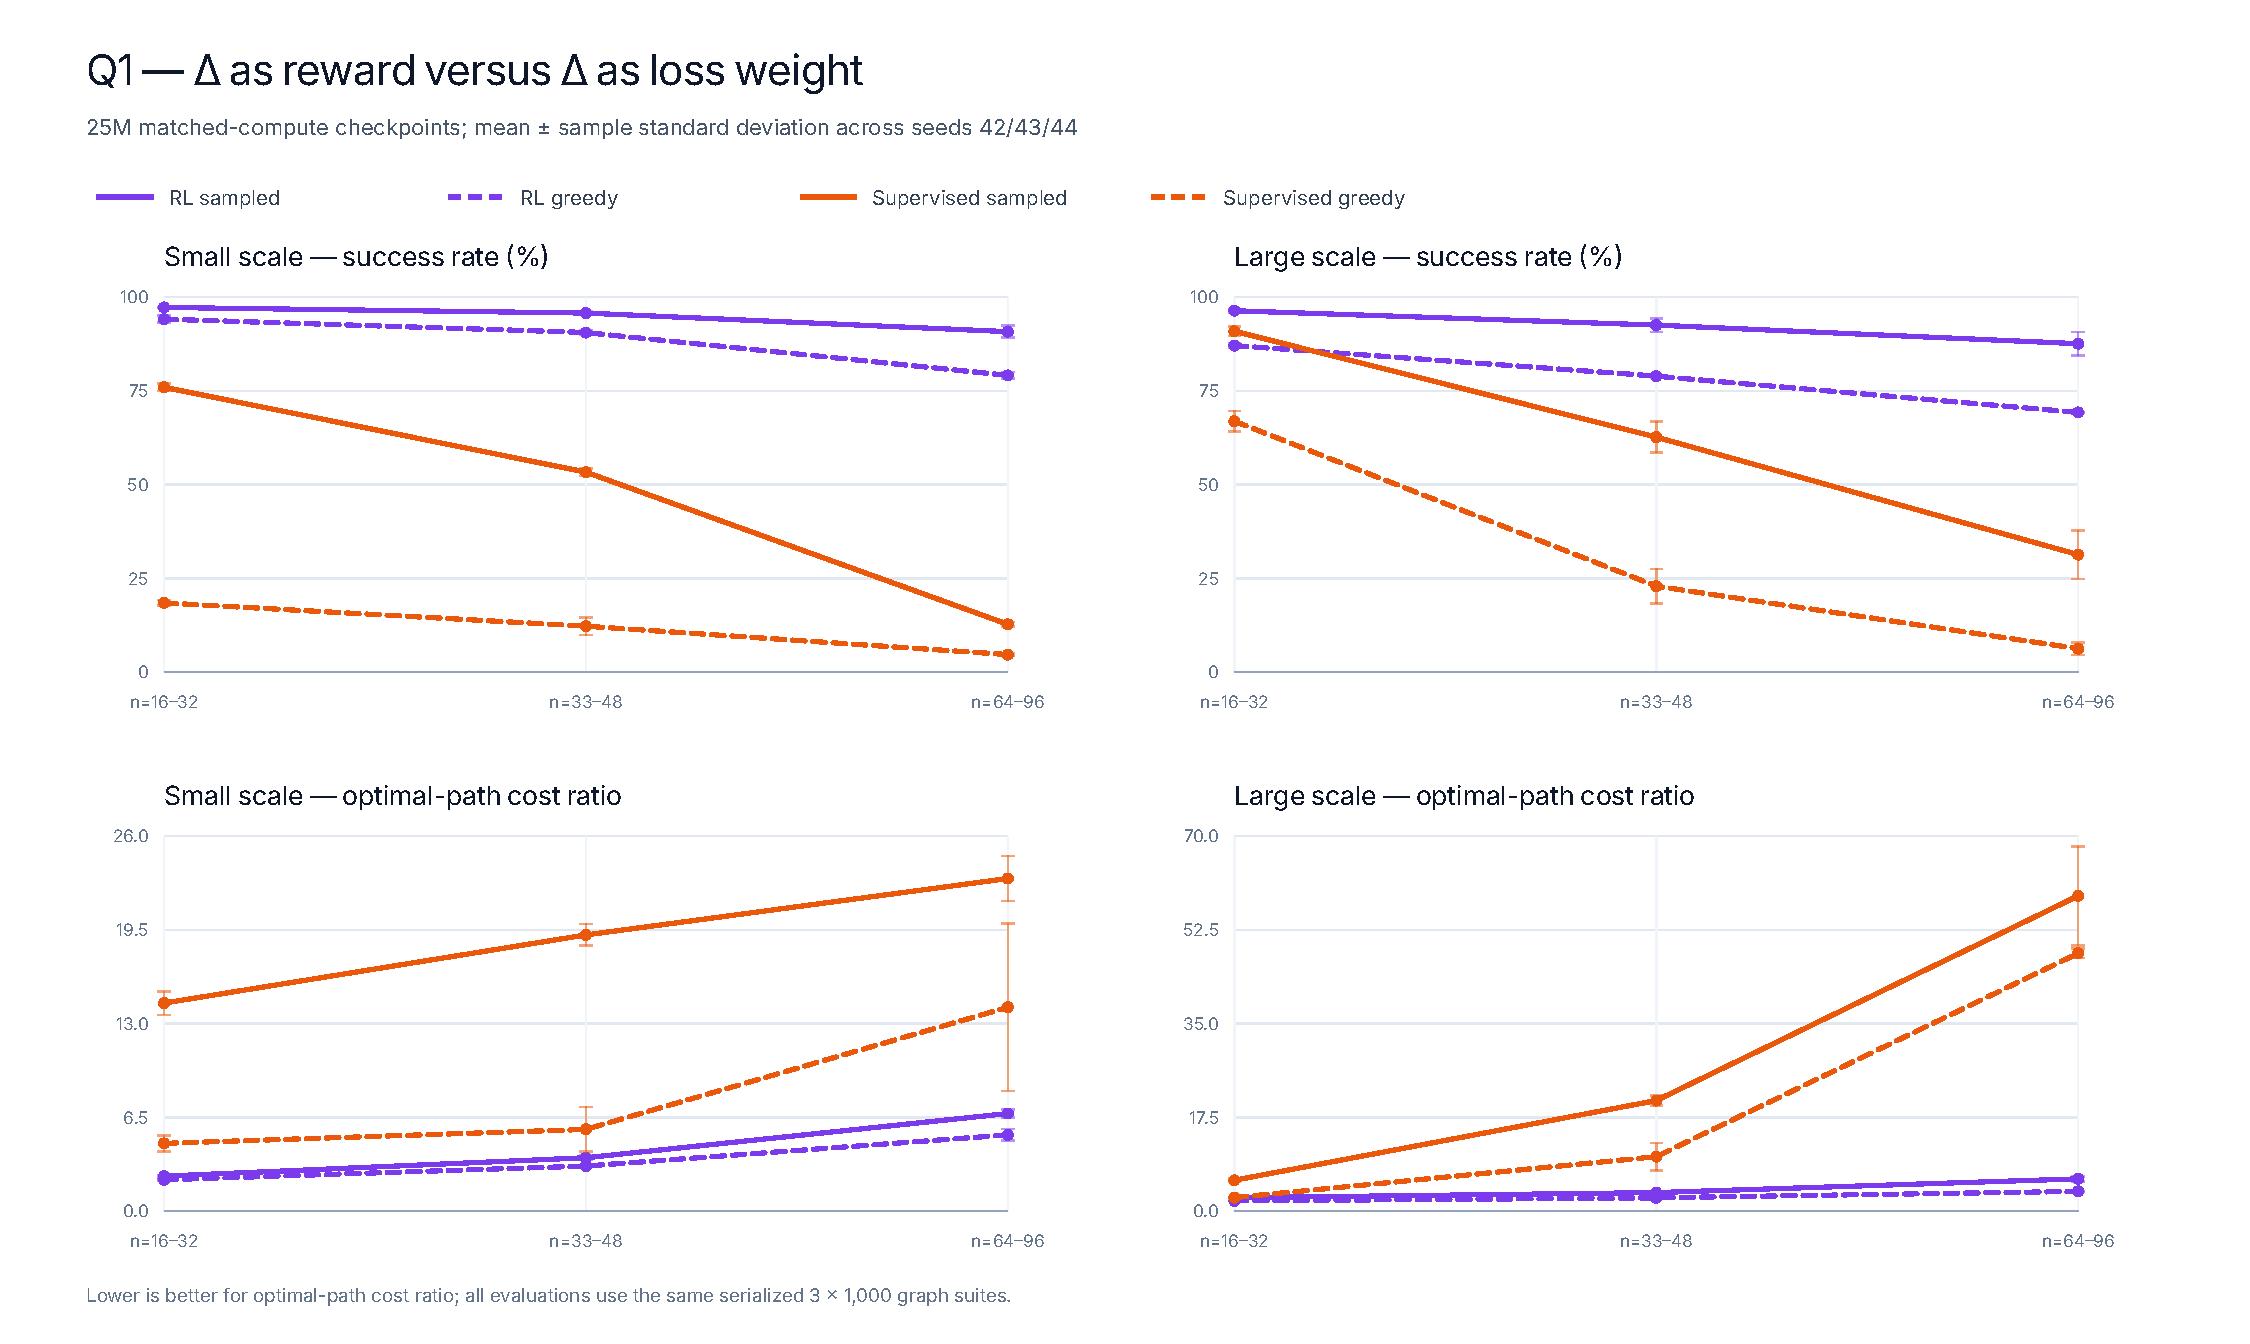
\includegraphics[width=\textwidth]{q1-cross-paradigm.pdf}
\caption{Cross-paradigm Q1 results over all matched parameter scales, budgets,
suites, and decoding modes.  Error bars are sample standard deviations across
training seeds 42, 43, and 44.}
\label{fig:q1}
\end{figure*}

\subsection{Gate and interpretation}

The Q1 gate passes broadly rather than through a selected outlier.  Across all
matched cells, 24 exceed the strict five-point absolute success threshold, 24
exceed the strict 0.5 optimality-gap threshold, and six train-to-far
degradation comparisons have non-overlapping seed ranges.  The maximum
absolute success difference is 80.60 points (small, 5M, train-scale, greedy);
the maximum gap difference is 52.82 (large, 25M, far-OOD, sampled).

The converged 20K-step supervised reference does not repair far-OOD behavior.
Its sampled success is 46.30\% at small scale and 29.40\% at large scale;
greedy success is 8.33\% and 7.00\%.  More optimization is therefore not a
simple explanation for the matched-checkpoint result.

The controlled interpretation is exposure to state distributions.  The
supervised learner grades expert-state decisions, whereas RL optimizes on
trajectories induced by its own mistakes and recoveries.  The experiment is
consistent with exposure bias, but does not isolate it from every difference
between PPO/Muon and soft-KL training.

\section{Q2: A Predeclared Shaping Phase Diagram}
\label{sec:q2}

The main grid trains an LSTM for 5M agent steps in 54 conditions: three rewards
(graded $\beta=1$, $\beta=0$, binary backward penalty), three horizons
($4n$, $2n$, $1.25n$), two fixed start regimes ($n=8$--16 and cold-start
$n=32$--64), and three seeds.  The complete grid is then repeated with goal
bonuses 1 and 0, giving 162 trainings.  Each checkpoint is evaluated by sampled
decoding on 1,000 shared held-out graphs.

\begin{table}[t]
\centering
\caption{Q2 main grid at goal bonus 10.  Success is the three-seed mean; gap is
graded minus $\beta{=}0$.}
\label{tab:q2}
\small
\begin{tabular}{@{}lrrrr@{}}
\toprule
Start & Horizon & Graded & $\beta{=}0$ & Gap\\
\midrule
$n=8$--16 & $4n$ & 99.7 & 99.3 & 0.4\\
$n=8$--16 & $2n$ & 97.7 & 96.5 & 1.2\\
$n=8$--16 & $1.25n$ & 95.1 & 93.1 & 1.9\\
$n=32$--64 & $4n$ & 97.1 & 89.3 & 7.7\\
$n=32$--64 & $2n$ & 89.1 & 80.6 & 8.5\\
$n=32$--64 & $1.25n$ & \textbf{83.2} & 71.7 & \textbf{11.5}\\
\bottomrule
\end{tabular}
\end{table}

Table~\ref{tab:q2} shows a coherent regime map.  Larger cold-start graphs create
most of the separation, and tighter horizons strengthen it.  In the strongest
cell, seed ranges separate cleanly (82.1--85.2\% graded versus
70.3--74.3\% control), but the 11.5-point mean gap remains below the declared
15-point threshold.  Binary shaping also reaches 83.2\%, equal to graded at
reported precision; direction matters, but exact regret magnitude is not
uniquely necessary.

Removing the terminal bonus does not uncover a hidden effect.  The strongest
gaps are 12.2 points at bonus 1 and 12.4 at bonus 0.  The latter is not
reward-free: $\beta=0$ still pays edge and step costs, and goal termination
removes future penalties.  All 162 conditions have zero invalid-action rate.

\begin{figure*}[t]
\centering
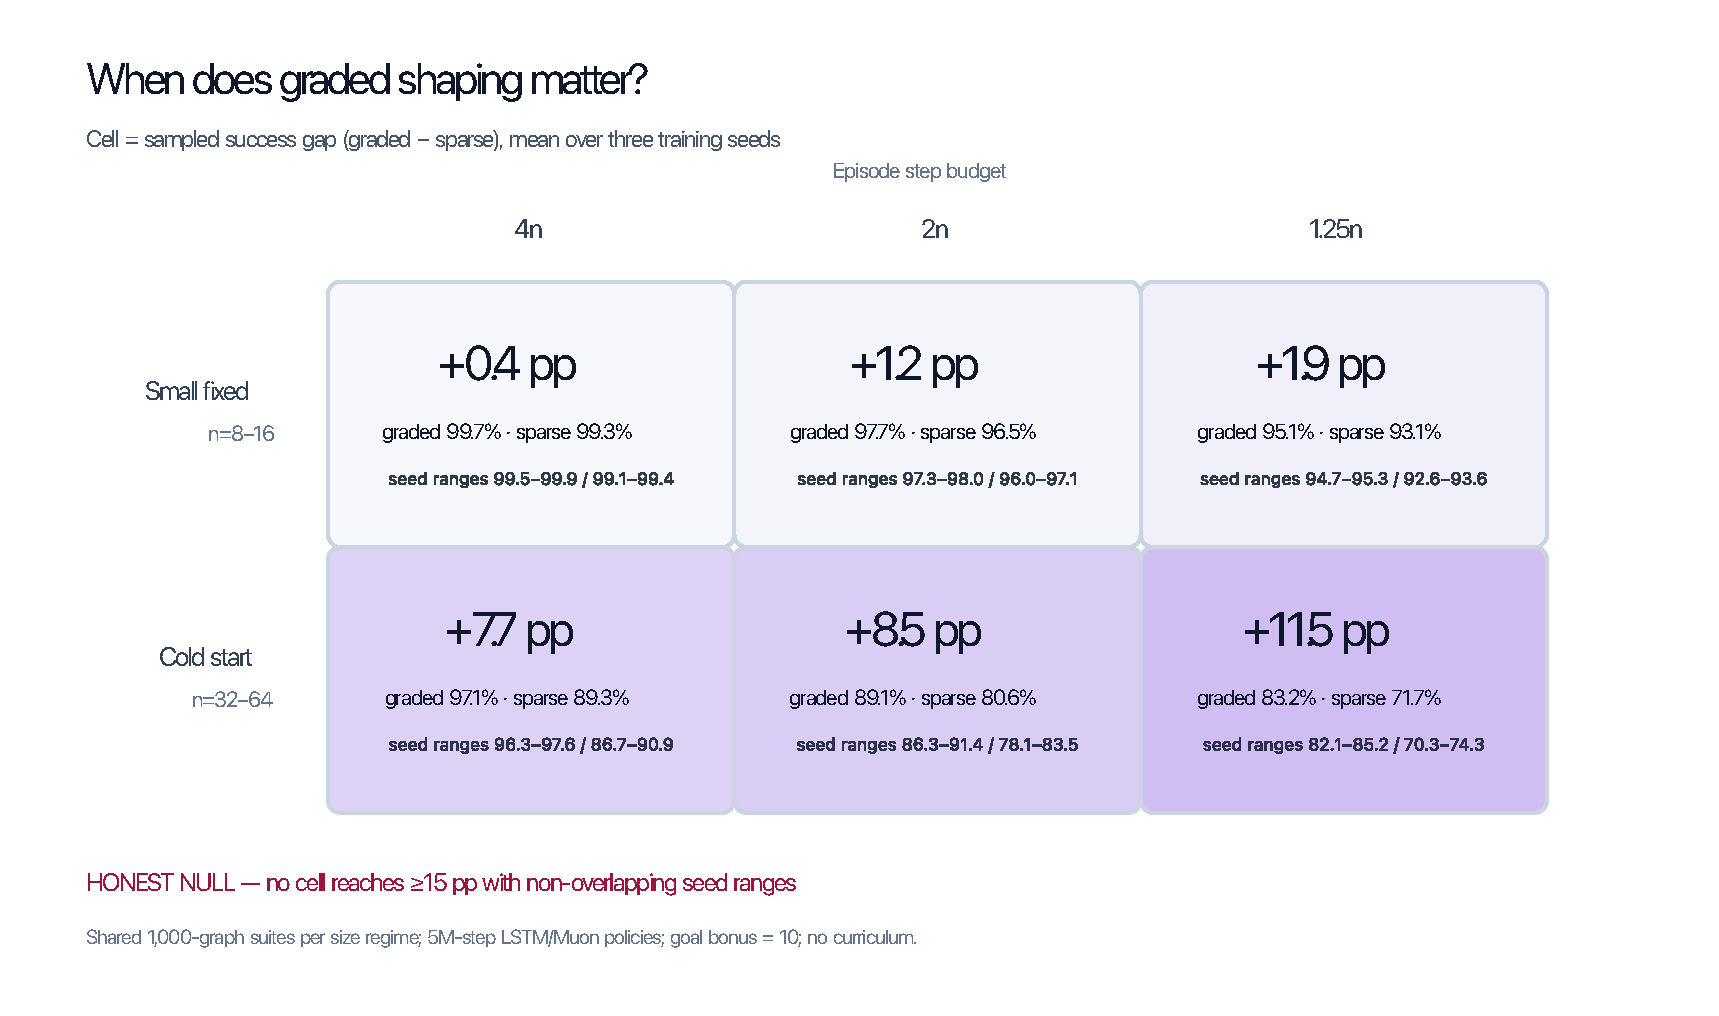
\includegraphics[width=0.88\textwidth]{q2-phase-diagram.pdf}
\caption{Q2 shaping phase diagram.  Shaping helps systematically in large
cold-start, tight-horizon regimes, but no goal-bonus level reaches the
predeclared 15-point gate.}
\label{fig:q2}
\end{figure*}

Q2 is therefore an \emph{honest null}.  The evidence does not show that shaping
is useless; it bounds its effect under the tested optimization settings.
Curriculum and a generous horizon make the directional term nearly redundant
on small graphs, while harder initial states yield a repeatable sub-threshold
advantage.  No learning rate, optimizer, seed, or cell was retuned after seeing
the gate.

\section{Q3: Size Generalization and Decoding}
\label{sec:q3}

Nine policies---MLP, LSTM, and Transformer at three seeds---train for 5M steps
under the curriculum through $n=32$.  Each is evaluated on the same 1,000
graphs per size for
$n\in\{32,48,96,192,384,768\}$, with a $4n$ budget and both decoding rules.
The size feature is clipped at one above the declared $N_{\mathrm{cap}}=64$,
keeping every observation inside the training-time box.

\begin{table}[t]
\centering
\caption{Sampled-decoding success (\%) across graph size.  Values are
three-seed means; all learned policies train only through $n=32$.}
\label{tab:q3success}
\small
\begin{tabular}{@{}rrrrr@{}}
\toprule
$n$ & Random & MLP & LSTM & Transf.\\
\midrule
32  & 87.67 & 96.37 & 98.30 & 94.33\\
48  & 85.83 & 94.83 & 96.73 & 85.70\\
96  & 84.97 & 93.13 & 95.83 & 75.30\\
192 & 85.43 & 91.50 & 94.50 & 66.03\\
384 & 81.73 & 90.97 & 94.00 & 62.83\\
768 & 82.67 & \textbf{90.93} & \textbf{93.57} & 56.07\\
\bottomrule
\end{tabular}
\end{table}

Q3 passes at $n=384$, twelve times the maximum training size:
MLP and LSTM remain above 90\%, while the Transformer falls to 62.83\%.
At $n=768$, the separation widens to 90.93\%, 93.57\%, and 56.07\%.
The result is not uniform Transformer inferiority.  On successful $n=768$
episodes its optimality gap is 22.54, less than half the MLP's 50.11 and the
LSTM's 55.32.  The Transformer learns a more efficient but brittle policy;
the simpler models preserve high-probability reachability with increasingly
expensive walks.

\begin{figure*}[t]
\centering
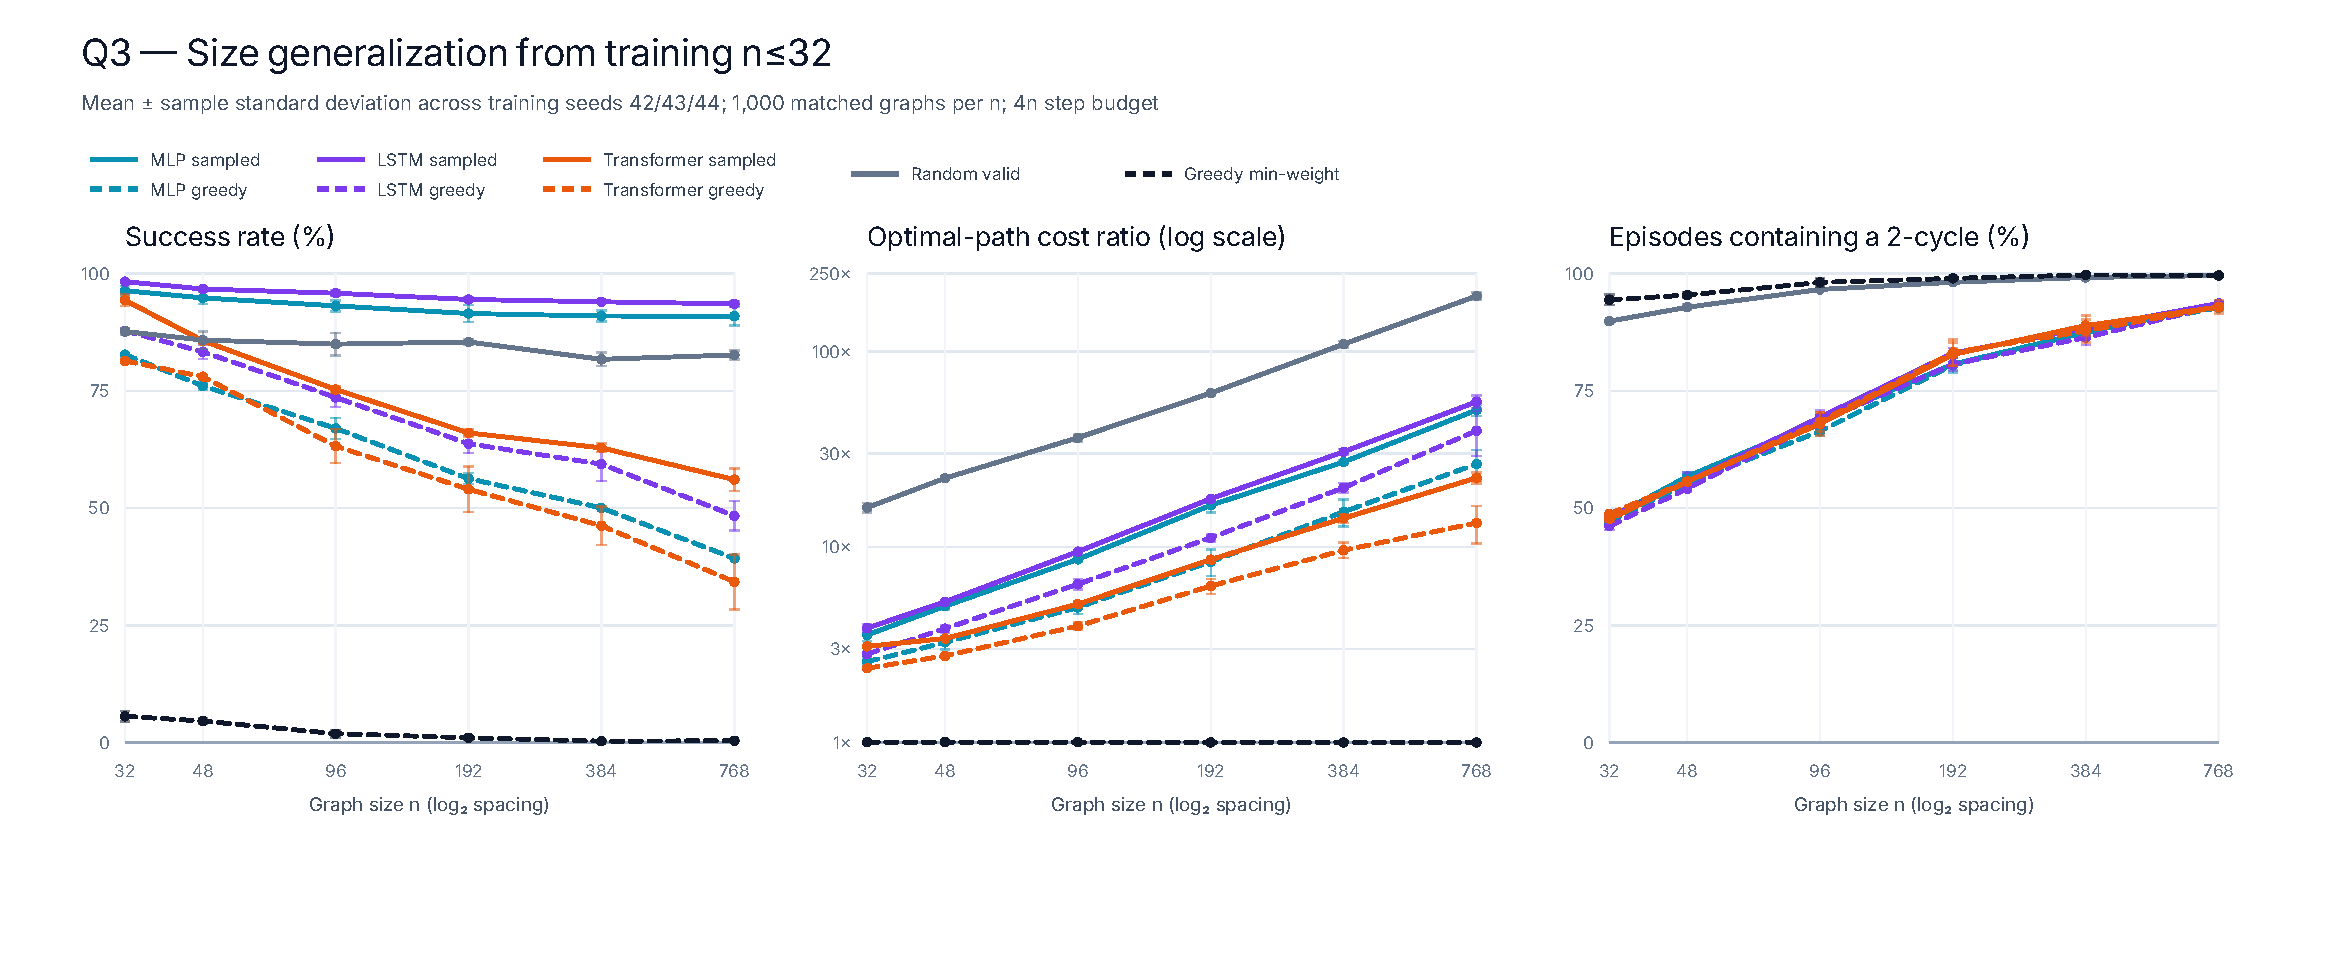
\includegraphics[width=\textwidth]{q3-size-generalization.pdf}
\caption{Q3 size generalization.  Sampled MLP/LSTM preserve reachability far
beyond training size, whereas the Transformer trades success for lower
successful-path cost.  Greedy decoding exposes a shared cycle pathology.}
\label{fig:q3}
\end{figure*}

\subsection{Sampling escapes cycles; it does not solve them}

At $n=768$, greedy success is only 39.27\% for MLP, 48.33\% for LSTM, and
34.27\% for Transformer.  Sampled success is higher by 21.8--51.7 points, yet
93.40\%, 93.67\%, and 92.90\% of sampled episodes still contain a two-cycle.
Sampling is a stochastic escape mechanism, not evidence that the underlying
deterministic controller is cycle-free.

Classical controls make the distinction concrete.  Uniform random valid walks
retain 82--88\% success through $n=768$ under the generous $4n$ horizon, but
their successful-path gap rises from 15.89 at $n=32$ to 192.27 at $n=768$ and
two-cycle incidence reaches 99.60\%.  Greedy minimum-edge selection has gap
approximately 1 on its rare successes, but success falls from 5.57\% to
0.37\%.  Reachability, efficiency, and local cycling are separate axes.

\section{Discussion}
\label{sec:discussion}

\paragraph{Information and interface are not interchangeable.}
Q1 controls the graph distribution, local observation, regret definition,
parameter scale, and approximate model compute.  Its OOD gap suggests that
training on self-induced trajectories is valuable when early errors move the
policy away from expert states.  However, PPO, Muon dynamics, and the number of
distinct encountered states remain part of the treatment; the result is not a
general causal decomposition of exposure bias.

\paragraph{Policy invariance does not predict learning utility.}
The identity at $\beta=1$ is exact, but the usual PBRS theorem does not promise
faster PPO learning.  Moreover, PPO uses $\gamma=0.995$ while the implemented
potential difference is undiscounted.  Q2 is informative precisely because it
shows that an exact local direction can become redundant under curriculum,
edge costs, goal termination, and a loose horizon.

\paragraph{Sampling is an algorithmic choice.}
Reporting only argmax or only sampled decoding would yield incompatible
stories.  Supervised sampling often rescues policies whose greedy rollouts
fail, but the rescued paths can be extremely inefficient.  In Q3, sampling
rescues learned policies from two-cycles without eliminating the cycles.  A
decoding rule is therefore part of a learned executor, not merely a display
setting.

\paragraph{Success is not shortest-path execution.}
The random-valid baseline rules out interpreting high reachability as
Dijkstra-like behavior.  Conversely, the min-edge baseline shows that
near-optimal conditional path cost can coexist with near-total failure.  Claims
about learned search require the joint metric vector: success, cost,
directionality, cycles, and horizon.

\section{Limitations}

The graph generator, local feature set, $K=8$ truncation, and positive edge
weights define a specific distribution.  The policies do not receive global
graph structure, and the comparison does not rank RL and supervised neural
algorithmic reasoning in general.  Parameter counts and estimated model MACs
are closely matched, but wall-clock, optimizer work, and distinct-state counts
are not.

Three training seeds support robust practical-effect comparisons but not
fine-grained distributional inference.  Gate counts are not independent
hypothesis tests: cells share training checkpoints and suite construction.
Optimality gap is conditional on success and can be unstable when few episodes
terminate.  The fixed sampling temperature is part of the declared protocol;
a wider temperature sweep should be treated as a decoding ablation, not as a
newly tuned headline.

The $4n$ horizon permits random exploration to succeed surprisingly often.
This is useful as a control but weakens any success-only claim.  Stronger
algorithmic evidence would require tighter horizons, explicit memory controls,
different graph families, or evaluation that directly prices exploration.

\section{Conclusion}

Exact Dijkstra regret is useful, but how it reaches the learner matters.  In
this local graph-walking task, RL trained from $-\dlt/\wmax$ is markedly more
robust than soft-KL teacher forcing on larger held-out graphs at matched model
scale and estimated compute.  Reward shaping itself produces a coherent but
sub-threshold finite-budget advantage once curricula and horizons are
controlled.  Simple recurrent and feed-forward policies preserve sampled
reachability far beyond training size, yet all learned controllers retain
severe cycle and path-efficiency failures.

The strongest supported conclusion is therefore not that one paradigm or
architecture executes Dijkstra.  Robust learned search is a joint property of
the learning interface, induced state distribution, decoding rule, horizon,
and path efficiency.  Fixed suites, predeclared gates, classical controls, and
honest nulls are necessary to see that distinction.

\section*{Reproducibility Statement}

The merged Q1 dataset contains exactly 72 RL rows and 108 supervised rows;
every row has invalid-action rate zero.  Q2 contains 162 fixed-suite
conditions, also with zero invalid actions.  Q3 contains 108 learned evaluation
conditions plus classical controls.  All checkpoints, curves, manifests, and
evaluations encode their training seed.  Machine-readable aggregates, complete
tables, plotting scripts, and suite manifests accompany the manuscript.

\appendix
\section{Complete 5M Q1 Snapshot}

Table~\ref{tab:q1five} reports the lower-budget matched comparison.  It
reproduces the qualitative ordering of the 25M result without selecting a
favorable suite or decoding rule.

\begin{table*}[t]
\centering
\caption{Q1 at the 5M compute match.  Entries are success (\%) / optimality
gap / backward rate (\%), averaged over three seeds.}
\label{tab:q1five}
\footnotesize
\resizebox{\textwidth}{!}{%
\begin{tabular}{@{}lllccc@{}}
\toprule
Scale & Learner & Decode &
Train scale $n{=}16$--32 & Near OOD $n{=}33$--48 & Far OOD $n{=}64$--96\\
\midrule
Small & RL & greedy
 & 90.23 / 2.31 / 20.75 & 86.10 / 3.41 / 26.28 & 76.57 / 5.59 / 33.94\\
Small & RL & sampled
 & 98.13 / 3.05 / 20.43 & 97.40 / 4.74 / 26.86 & 95.40 / 8.87 / 33.35\\
Small & supervised & greedy
 & 9.63 / 3.07 / 44.23 & 6.50 / 1.35 / 45.69 & 3.23 / 1.77 / 47.28\\
Small & supervised & sampled
 & 81.40 / 14.38 / 38.78 & 72.57 / 21.57 / 41.80 & 67.77 / 36.78 / 44.14\\
\midrule
Large & RL & greedy
 & 87.60 / 1.96 / 20.64 & 78.73 / 2.42 / 26.66 & 67.00 / 3.53 / 33.98\\
Large & RL & sampled
 & 96.00 / 2.42 / 19.91 & 89.27 / 3.20 / 26.22 & 77.40 / 4.63 / 33.69\\
Large & supervised & greedy
 & 34.50 / 3.66 / 35.04 & 14.20 / 10.13 / 44.84 & 4.10 / 15.71 / 47.26\\
Large & supervised & sampled
 & 82.23 / 10.19 / 33.63 & 59.90 / 20.84 / 42.36 & 24.50 / 48.62 / 46.22\\
\bottomrule
\end{tabular}}
\end{table*}

\section{Suite and Seed Integrity}

The Q1 serialized suites use 1,000 graphs each.  Their SHA-256 digests and the
graph-generator implementation digest are:
\begin{center}
\begin{tabular}{@{}ll@{}}
\textbf{train} & \texttt{\scriptsize c848ff46125e1cf6998a505a094a6efe}\\[-1pt]
 & \texttt{\scriptsize b3e170091a67b7b241623a5a42727463}\\[1pt]
\textbf{near} & \texttt{\scriptsize dba06cb89c76e674abc8d960ace768ec}\\[-1pt]
 & \texttt{\scriptsize a1ac13db2d2111eb724f8a8847b6145c}\\[1pt]
\textbf{far} & \texttt{\scriptsize d93e4b086a054660f3e40d0e8d7b0170}\\[-1pt]
 & \texttt{\scriptsize abb35569bae29e6d8d7a359207d83bbc}\\[1pt]
\textbf{generator} & \texttt{\scriptsize 5a9de1c8ff44c693f797cb09c50d66b2}\\[-1pt]
 & \texttt{\scriptsize 374a810033b1163767c7ce8f7f3cd9f5}\\
\end{tabular}
\end{center}
Hashes were verified before remote evaluation and after local retrieval.
Equal-seed 16,384-step checks produce tensor-identical checkpoints and
identical non-timing curves; changing the seed changes model initialization.

\section{Environment Vectorization}

The environment precomputes each node's exposed neighbor table at reset and
uses NumPy gathers for selected destinations, weights, potential changes,
rewards, visited-state updates, and observations.  The Python loop remains only
for terminated rows, preserving reset and graph-RNG order.

\begin{table}[h]
\centering
\caption{Vectorization benchmarks on 1,024 environments.}
\label{tab:vector}
\small
\begin{tabular}{@{}lrrr@{}}
\toprule
Workload & Scalar SPS & Vector SPS & Speedup\\
\midrule
Step kernel & 267,751 & 5,013,644 & 18.72$\times$\\
Full env. & 157,686 & 316,578 & 2.01$\times$\\
PPO, 500K & 73,867 & 96,141 & 1.30$\times$\\
\bottomrule
\end{tabular}
\end{table}

Two 120-step public-output traces, one graded and one binary, remain
byte-identical across the scalar and vectorized implementations.  Exact graph
generation and Dijkstra at reset account for roughly 74\% of the remaining
full-environment time.  We therefore report the 1.30$\times$ PPO improvement
rather than presenting the 18.72$\times$ kernel result as training speed.

\section{Execution Audit}

Q1 ran on a GTX 1080 (compute capability 6.1) using an official CUDA 12.6
PyTorch wheel.  At most two GPU processes ran concurrently under reduced
priority, with OMP, MKL, and OpenBLAS thread counts capped at one.  Training and
evaluation logs were retained per seed.  Two first attempts failed before
model execution because \code{/usr/bin/time} was unavailable; each traceback
was retained and each wrapper was retried exactly once with shell epoch timing.
No scientific crash was silently rerun.

The remote suite hashes matched the pinned local values.  Artifacts were
streamed back and counted before remote deletion: 24 RL files, 54 supervised
files, and 12 evaluation JSONs.  Bulk remote artifacts and the shared virtual
environment were removed after retrieval; raw logs were retained.

\balance
{\scriptsize
\setlength{\bibsep}{1pt plus 0.2ex}
\bibliographystyle{plainnat}
\bibliography{references}
}

\end{document}
